% -----------------------------------------------
% Template for ISMIR Papers
% 2021 version, based on previous ISMIR templates

% Requirements :
% * 6+n page length maximum
% * 10MB maximum file size
% * Copyright note must appear in the bottom left corner of first page
% * Clearer statement about citing own work in anonymized submission
% (see conference website for additional details)
% -----------------------------------------------

\documentclass{article}
\usepackage[T1]{fontenc} % add special characters (e.g., umlaute)
\usepackage[utf8]{inputenc} % set utf-8 as default input encoding
\usepackage{ismir,amsmath,cite,url}
\usepackage{amsmath, amssymb, amsfonts, amsthm}
\usepackage{algorithm}% http://ctan.org/pkg/algorithms
\usepackage{algpseudocode}% http://ctan.org/pkg/algorithmicx
\usepackage{mathtools}
\usepackage{graphicx}
\usepackage{color}


\usepackage{lineno}
\linenumbers

% Title. Please use IEEE-compliant title case when specifying the title here,
% as it has implications for the copyright notice
% ------
\title{Traveling Salesperson Tunes}

% Note: Please do NOT use \thanks or a \footnote in any of the author markup

% Single address
% To use with only one author or several with the same address
% ---------------
%\oneauthor
% {Names should be omitted for double-blind reviewing}
% {Affiliations should be omitted for double-blind reviewing}

% Two addresses
% --------------
%\twoauthors
%  {First author} {School \\ Department}
%  {Second author} {Company \\ Address}

% Three addresses
% --------------\input{ISMIR2021_paper.tex}

\twoauthors
  {Alexa Lewis} {Ursinus College Mathematics \\ {\tt author1@ismir.edu}}
  {Christopher J. Tralie} {Ursinus College Mathematics And Computer Science \\ {\tt ctralie@alumni.princeton.edu}}

% Four or more addresses
% OR alternative format for large number of co-authors
% ------------
%\multauthor
%{First author$^1$ \hspace{1cm} Second author$^1$ \hspace{1cm} Third author$^2$} { \bfseries{Fourth author$^3$ \hspace{1cm} Fifth author$^2$ \hspace{1cm} Sixth author$^1$}\\
%  $^1$ Department of Computer Science, University , Country\\
%$^2$ International Laboratories, City, Country\\
%$^3$  Company, Address\\
%{\tt\small CorrespondenceAuthor@ismir.edu, PossibleOtherAuthor@ismir.edu}
%}

% For the author list in the Creative Common license, please enter author names. 
% Please abbreviate the first names of authors and add 'and' between the second to last and last authors.
\def\authorname{A. Lewis and C. Tralie}

% Optional: To use hyperref, uncomment the following.
%\usepackage[bookmarks=false,pdfauthor={\authorname},pdfsubject={\papersubject},hidelinks]{hyperref}
% Mind the bookmarks=false option; bookmarks are incompatible with ismir.sty.

\sloppy % please retain sloppy command for improved formatting

\graphicspath{{../figures/}}

\begin{document}

%
\maketitle
%
\begin{abstract}
  

\end{abstract}
%
\section{Introduction}\label{sec:introduction}




\section{Stipple Tunes}

To hide images in audio, we first turn to an intermediate representation: the {\em stipple pattern}.  This is a collection of dots that resembles an image.  We use the technique of Secord \cite{secord2002weighted}, which 

\begin{figure}
  \centering
  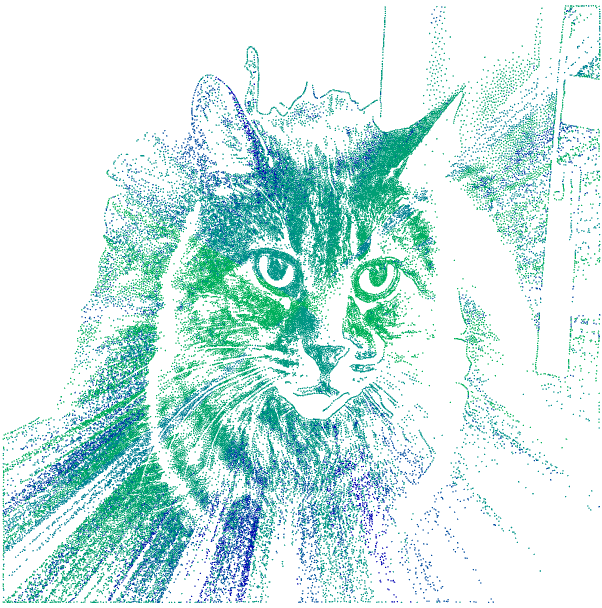
\includegraphics[width=0.8\columnwidth]{laylaViterbiStipple.png}
  \caption{A stipple tune on Layla the cat, using a 30 second clip from Eric Clapton's ``Layla,'' created from a stipple with 100,000 points.}
  \label{fig:laylaViterbiStipple}
\end{figure}


\algrenewcommand\algorithmicindent{0.8em}%
\begin{algorithm}
  \caption{Stipple Tunes Algorithm}

  \begin{algorithmic}[1]
    \Procedure{StippleTune}{$Z$, $x$, na, win, tw} \Comment{$Z$ is stipple, $x$ is audio samples, {\em na} is number of discrete angle states, {\em win} is number of samples between angle states, and {\em tw} is amount by which angle can jump each step}
    \State $N \gets \text{len}(x)$ \Comment{Number of audio samples}
    \State $Y \gets x + ix$
    \State Setup a KDTree {\em tree} for fast NN queries on $Z$
    \State $M \gets \text{ceil}(N / \text{win})$
    \State $C[i, 0] \gets 0, C[i, j > 1] \gets \infty$ \Comment{$na \times M$ Cumulative cost matrix}
    \State $I[i, j] \gets 0$ \Comment{$na \times M$ backpointers to best preceding state}
    \For{$t = 2:M$}
        \For{$j = 1:na$}
            \State $\theta_j \gets 2 \pi j / \text{na}$
            \For{$k = j-\text{tw}:j-1 \mod \text{na}$}
                \State $\theta_k \gets 2 \pi k / \text{na}$ \label{lst:line:interpolate}
                \State Let $\theta_{\ell} \gets \theta_j + (\theta_k-\theta_j)/\text{win}$ 
                \State $d \gets \sum_{\ell = 1}^{\text{win}} \text{tree.query}(Y[\text{win}*t + \ell] e^{i \theta_{\ell}})$ \Comment{Sum nearest neighbors of all points}
                \If{$C[k, t-1] + d < C[j, t]$}
                    \State $C[j, t] \gets C[k, t-1] + d$ 
                    \State $I[j, t] \gets k$  \Comment{Remember optimal transition}
                \EndIf
            \EndFor
        \EndFor
    \EndFor \\
    \State Backtrace $I$ to obtain the optimal sequence of angle states
    \State Linearly interpolate between each angle state (line~\ref{lst:line:interpolate}) to compute $\theta[k], k = 1 \text{ to } N$ 
    \State Let $X_k$ be the nearest neighbor in $Z$ to $Y_k e^{i \theta[k]}$, using {\em tree} to speed up queries \\
    \Return $X$
    \EndProcedure
  \end{algorithmic}
  \label{alg:stippletunes}
\end{algorithm}

We turn a single channel audio stream $x[j]$ into a 2D curve by simply repeating the channel twice: one for each coordinate.  From there, a simple idea is to find the nearest neighbor in the stipple pattern to each 2D audio point $(x[j], x[j])$.  However, this has an immediate drawback since the curve simply moves back and forth along the line $y=x$, so nearest neighbors would concentrate near this line.  To encourage the algorithm to explore points away from this line, we slowly rotate the line and sweep the entire stipple.



Formally, let $Y[j] = x[j] + i x[j]$ be an embedding of $(x[j], x[j])$ in the complex plane, and similarly embed the stipple $Z$ in the complex plane.  Then, we introduce a hidden state $\theta[j]$ so that we actually find the nearest neighbor from the points $Y_{\theta}[j] = Y[j] e^{i \theta[j]}$ to the stipple pattern $Z$.  The effect of $\theta[j]$ is to pan between the left and right audio channels, and snapping $Y_{\theta}[j]$ to the nearest point in the stipple can be thought of an unusual form of quantization.  

% \footnote{Of course, a probability can always be converted to a ``distance'' via a negative log}



Crucially, we encourage the line to move and sweep the whole image by forcing $\theta[j+1] > \theta[j] + \epsilon$ for some $\epsilon > 0$.  We can solve for the hidden states $\theta[j]$ using the Viterbi algorithm.  Rather than maximizing a probability, as in the traditional application of Viterbi to HMMs, we seek to {\em minimize} the sum of nearest neighbor distances.  In this way, our application is similar in spirit to corpus-based concatenative synthesis \cite{schwarz2007corpus}, where the ``corpus'' is simply the stipple pattern.  Algorithm~\ref{alg:stippletunes} provides more details. In practice, we discretize $\theta$ by a factor $win$ coarser than audio sample rate to keep the Viterbi algorithm tractable.  We also discretize the possible rotation angles to $na$, and we force adjacent angle states to be between $1$ and $tw < na$ of each other so that adjacent angles have to change, but not by an arbitrary amount.  Figure~\ref{fig:laylaViterbiStipple} shows an example of mapping a stipple of a special cat named Layla to a 30 second clip from Eric Clapton's ``Layla,'' using $na=60$, $win=f_s=44100$, and $tw=10$.  Since $win$ is the sample rate $f_s$, we only have one state per second, but we find this is enough to get a good sweep through the stipple.





% For bibtex users:
\bibliography{writeup}

\end{document}

